\documentclass[11pt]{article}

\usepackage[margin=1in]{geometry}
\usepackage[T1]{fontenc}
\usepackage{lmodern}
\usepackage{amsmath,amssymb}
\usepackage{graphicx}
\usepackage{booktabs}
\usepackage{caption}
\usepackage{setspace}
\usepackage[authoryear,round]{natbib}
\usepackage{xcolor}
\usepackage[colorlinks=true,linkcolor=blue!50!black,citecolor=blue!50!black,urlcolor=blue!50!black]{hyperref}
\usepackage{float}

\captionsetup{labelfont=bf,font=small,justification=centering}
\setstretch{1.25}
\setlength{\parskip}{0.35em}
\renewcommand{\thetable}{\Roman{table}}

\newcommand{\tabnote}[1]{\par\vspace{0.3em}\begin{minipage}{\linewidth}\footnotesize\setstretch{1.0}#1\end{minipage}}

\begin{document}

\begin{titlepage}
\begin{center}
{\LARGE\bfseries Crowded Carry: Crash Risk in\\[0.25em] Foreign Exchange and Crypto Carry Trades\par}
\vspace{1.5em}
{\large Amir Kermani \qquad Reza Zamani \qquad Paraj Goyal\footnote{Haas School of Business, University of California, Berkeley. This paper was written for MFE 230GB (Currency Markets). Data, code, and all results are available at \url{https://github.com/rezazamani2329/currency-crypto-carry}. Use of AI tools is documented in the repository's \texttt{ai\_log.md}. All errors are our own.}\par}
\vspace{1em}
{\large October 2026\par}
\end{center}

\vspace{2em}
\begin{abstract}
\noindent
Do carry trades crash when they are crowded? We study the question in two markets with the same economics but very different investors: G10 currencies (1999--2026) and crypto perpetual futures on Binance (2020--2026). In foreign exchange, a dollar-neutral carry strategy earns a net Sharpe ratio of 0.37, has a correlation of 0.82 with the Lustig--Roussanov--Verdelhan carry factor, and loses when equity volatility rises (volatility beta of $-1.55$, $t=-3.7$); its alpha is insignificant once dollar and volatility risk are controlled for. Crowding measured from CFTC speculator positions is a modest warning sign: carry earns 0.02\% in the month after a crowded reading against 0.30\% otherwise, and halving exposure when crowded raises the out-of-sample Sharpe ratio from 0.27 to 0.32. The filter does not avoid the largest crash, however, because 2008 began from a non-crowded reading. In crypto, shorting coins with the highest funding rates and buying those with the lowest collects about 8.5\% a year in funding but earns only 4.1\% net with 30\% volatility (Sharpe 0.14). The strategy has no Bitcoin exposure, and its crashes are coin-specific: the worst week ($-27$\%) came from being long Terra (LUNA), which traders were crowding to short. FX and crypto carry are nearly uncorrelated (0.11). Our answer is ``partly yes'': crowding makes carry weaker, but it does not predict the biggest crashes.
\end{abstract}

\vspace{1em}
\noindent\textbf{JEL classification:} F31, G12, G15, G23

\noindent\textbf{Keywords:} carry trade, crash risk, crowding, CFTC positioning, cryptocurrency, perpetual futures, funding rates
\end{titlepage}

\setcounter{page}{1}

%==========================================================
\section{Introduction}
%==========================================================

Uncovered interest parity (UIP) says that a currency with a high interest rate should depreciate by exactly the interest differential, so that borrowing in a low-rate currency and lending in a high-rate one earns nothing on average. Since \citet{HansenHodrick1980} and \citet{Fama1984}, a large literature has shown the opposite: high-yield currencies tend to appreciate, or depreciate by less than the rate gap, and the carry trade earns a sizeable premium. The leading explanation is that this premium compensates for crash risk. Carry trades go ``up the stairs and down the elevator'': they earn small steady gains most of the time and lose a large amount in a few weeks when global risk appetite falls \citep{BrunnermeierNagelPedersen2008, Menkhoff2012, Farhi2016}.

\citet{BrunnermeierNagelPedersen2008} add a second ingredient. Crashes are worse when speculators hold large positions in the trade, because a funding shock forces them to unwind together. Crowding is therefore a natural candidate for predicting \emph{when} carry will crash. This paper asks a simple question: \textbf{do carry trades crash when they are crowded?}

We study the question in two markets that share the economics of carry but differ in who trades. The first is the classic G10 currency market, where carry is the gap between short-term interest rates and crowding can be measured from the Commodity Futures Trading Commission (CFTC) report on speculators' futures positions. The second is the market for crypto perpetual futures. A perpetual future has no expiry; instead, longs and shorts exchange a \emph{funding rate} every eight hours that keeps the futures price close to spot. When leveraged traders crowd into long positions, longs pay shorts. The funding rate is therefore both the crypto analogue of an interest-rate differential and a direct measure of crowded leveraged demand.

We build two pre-specified, dollar-neutral strategies. Strategy~A is a monthly G10 carry strategy that buys the two currencies with the highest three-month interest rates and sells the two with the lowest, and halves its positions when CFTC positioning shows that its longs are crowded long and its shorts crowded short. Strategy~C is a weekly crypto carry strategy that shorts the third of coins with the highest seven-day funding and buys the third with the lowest. All parameters, the in-sample/out-of-sample split, and transaction costs were fixed before any backtest was run.

We find four main results. First, G10 carry earns a modest premium after costs (Sharpe ratio 0.37 over 1999--2026) and closely tracks the academic carry factor of \citet{LRV2011}, with a correlation of 0.82. Its losses line up with volatility shocks: in a regression on the dollar factor and equity-volatility innovations, the volatility beta is $-1.55$ ($t=-3.7$) and the alpha is not significant. This is the standard risk-based picture of carry.

Second, crowding is a modest but imprecise warning sign. In the month after a crowded reading, carry earns 0.02\% against 0.30\% after non-crowded months, and its returns are more negatively skewed. Halving exposure when crowded raises the out-of-sample Sharpe ratio from 0.27 to 0.32, and every setting in a robustness grid beats plain carry out of sample. Yet only 33 of 328 months were crowded, and the 2008 crash began from a non-crowded reading, so the maximum drawdown ($-37$\%) is the same with or without the filter.

Third, crypto funding carry collects real funding income of about 8.5\% a year, but price moves decide its performance. Net of costs it earns 4.1\% a year with 30\% volatility (Sharpe 0.14), losing in 2020--2023 and earning a Sharpe of 0.81 since 2024. The strategy has no Bitcoin exposure (beta $-0.02$), and its crashes are coin-specific. They arise in the mirror image of FX: because the strategy buys coins with the most negative funding, it ends up long whatever traders short hardest. In May 2022 that meant being long Terra (LUNA) into its collapse, which cost 27\% in a single week.

Fourth, FX and crypto carry are almost uncorrelated (0.11). A 50/50 mix scaled to equal volatility has lower volatility and a smaller drawdown than either strategy alone.

Our answer to the main question is therefore ``partly yes.'' Crowding makes carry weaker, but it does not predict the biggest crashes. In FX, crash risk is mainly compensation for exposure to global volatility, and positioning is only a modest overlay. In crypto, crowding tells you \emph{where} the danger is, in the coins with extreme funding on either side, rather than \emph{when} it will hit.

\paragraph{Related literature.}
Our paper connects three strands of work. The first documents the carry premium and explains it with risk. \citet{LustigVerdelhan2007} and \citet{LRV2011} show that a high-minus-low carry factor prices the cross-section of currency portfolios, and \citet{LRV2014} show that currency risk premia are countercyclical. \citet{Menkhoff2012} identify global FX volatility as the priced risk, \citet{Burnside2011} discuss peso problems, \citet{Jurek2014} studies crash-hedged carry, \citet{DanielHodrickLu2017} document carry drawdowns, and \citet{Farhi2016} model rare disasters. \citet{Koijen2018} show that carry predicts returns in many asset classes. We replicate the standard G10 result and its link to volatility risk.

The second strand studies crowding and forced unwinding. \citet{BrunnermeierPedersen2009} model the spiral between market liquidity and funding liquidity, \citet{Pedersen2009} describes how crowded trades crash when ``everyone runs for the exit,'' and \citet{Stein2009} discusses how crowding by sophisticated investors can destabilise prices. \citet{BrunnermeierNagelPedersen2008} show that speculator positions in currency futures predict carry crash risk, and \citet{Moskowitz2012} use the same CFTC data to study how speculators trade on trends. We turn this evidence into a simple, pre-specified trading rule and test it out of sample through 2026.

The third strand studies cryptocurrency returns. \citet{LiuTsyvinski2021} and \citet{LiuTsyvinskiWu2022} document the risk factors that explain crypto returns, \citet{He2022} describe the pricing of perpetual futures, and \citet{Schmeling2023} show that crypto carry, the futures--spot basis, reflects leveraged demand from retail investors and predicts crash risk. Our contribution is to treat the funding rate as both the carry signal and the crowding signal, to test it on a universe that keeps the coins that collapsed (Terra and FTX Token), and to compare it side by side with FX carry under the same design.

The rest of the paper is organised as follows. Section~\ref{sec:hyp} states the hypotheses. Section~\ref{sec:data} describes the data, and Section~\ref{sec:method} the strategies and methodology. Section~\ref{sec:fx} presents the FX results and Section~\ref{sec:crypto} the crypto results. Section~\ref{sec:comb} studies the combined portfolio, Section~\ref{sec:disc} discusses the results and their limitations, and Section~\ref{sec:concl} concludes.

%==========================================================
\section{Hypotheses}\label{sec:hyp}
%==========================================================

We split the main question into six research questions: (RQ1) whether G10 carry earns a premium after costs and reproduces the academic carry factor; (RQ2) whether crowding predicts weaker or more crash-prone carry; (RQ3) when FX carry loses money; (RQ4) whether crypto funding carry earns a premium and whether it comes from funding or from price moves; (RQ5) what drives crypto carry losses; and (RQ6) whether FX and crypto carry diversify each other. The corresponding hypotheses, written down before any backtest was run, are:

\begin{description}\setlength{\itemsep}{0.2em}
\item[H-A1.] G10 carry earns a positive expected excess return after transaction costs. The null is a zero expected return.
\item[H-A2.] Carry is weaker and more negatively skewed in the month after a crowded reading, so that cutting exposure when crowded raises the out-of-sample Sharpe ratio. The null is that next-month carry is the same after crowded and non-crowded months.
\item[H-A3.] Carry loses when volatility rises. The null is that carry returns are unrelated to volatility shocks.
\item[H-C1.] Shorting high-funding coins and buying low-funding coins earns a positive return after costs, mainly from the funding it collects.
\item[H-C2.] Because it is dollar-neutral, crypto carry has little exposure to Bitcoin, and its crashes are coin-specific rather than market-wide.
\item[H-D.] FX carry and crypto carry have low correlation, so a combined portfolio diversifies.
\end{description}

%==========================================================
\section{Data}\label{sec:data}
%==========================================================

All data are public and were downloaded on October 2, 2026. Table~\ref{tab:data} summarises the sources.

\begin{table}[!htbp]
\centering
\caption{Data Sources}\label{tab:data}
\small
\begin{tabular}{p{3.0cm}p{4.6cm}p{4.2cm}p{2.6cm}}
\toprule
Data & Source & Series and coverage & Used for \\
\midrule
FX spot rates & FRED (Federal Reserve H.10), daily, sampled at month-end & JPY, EUR, GBP, CHF, CAD, AUD, NZD against USD & Strategy A returns \\
3-month interbank rates & OECD via FRED, monthly & US, JP, euro area, UK, CH, CA, AU, NZ, DE & Strategy A signal \\
Speculator positions & CFTC Commitments of Traders, legacy futures-only, weekly & CME currency futures, 1986--2026 & Crowding signal \\
Crypto prices, volume, funding & Binance public archive, USDT-margined perpetuals & Daily candles and 8-hourly funding, 2020-01 to 2026-08 & Strategy C \\
Carry factor portfolios & \citet{LRV2011}, \textit{CurrencyPortfolios.xls} & Developed HML, dollar factor RX, volatility innovations, 1983--2021 & Validation and risk regressions \\
\bottomrule
\end{tabular}
\tabnote{This table lists the data used in the paper. FX spot rates are quoted in US dollars per unit of foreign currency. Interest rates are three-month interbank rates in percent per year. CFTC positions are non-commercial long and short futures positions and open interest. Crypto data cover twelve coins: BTC, ETH, BNB, XRP, ADA, DOGE, SOL, LTC, LINK, AVAX, LUNA, and FTT.}
\end{table}

\paragraph{Foreign exchange.}
Spot rates for JPY, GBP, CHF, CAD, AUD, and NZD begin in 1971 and EUR in 1999. Interest-rate histories are long for USD, EUR (Deutsche mark before 1999), GBP, CAD, AUD, and NZD, but begin only in 2002 for JPY and 1999 for CHF. Strategy~A therefore starts in May 1999 and runs to August 2026 (328 months).

\paragraph{CFTC positions.}
CFTC positions for CAD, CHF, EUR (Deutsche mark before 1999), GBP, and JPY are available from 1986, AUD from 1987, and NZD from 1999, with a gap in the NZD contract between 2000 and 2003. Before August 2000 the CFTC lists currency futures under the exchange name ``International Monetary Market'' rather than the Chicago Mercantile Exchange. Matching both names extends the positioning history back to 1986, which gives enough history for the 36-month z-score at the start of the strategy sample.

\paragraph{Crypto.}
The crypto universe contains twelve large coins: Bitcoin (BTC), Ethereum (ETH), BNB, XRP, Cardano (ADA), Dogecoin (DOGE), Solana (SOL), Litecoin (LTC), Chainlink (LINK), Avalanche (AVAX), Terra (LUNA), and FTX Token (FTT). LUNA and FTT, which collapsed in 2022, are deliberately kept to avoid survivorship bias. Funding is positive on most days: average annualised funding is 11.8\% for BTC, 13.9\% for ETH, and 14.7\% for XRP, and funding is positive on 81--88\% of days for the main coins. USDC is used only as a sanity check (its average funding is 0.04\% a year) and is not traded.

%==========================================================
\section{Methodology}\label{sec:method}
%==========================================================

\subsection{Strategy A: crowded G10 carry}

Let $S_{k,t}$ be the spot rate of currency $k$ in US dollars per unit and $i_{k,t}$ its three-month interest rate in percent per year. The monthly excess return of a long position in currency $k$ is
\begin{equation}
rx_{k,t} = \left(1+\frac{i_{k,t-1}}{1200}\right)\frac{S_{k,t}}{S_{k,t-1}} - \left(1+\frac{i_{US,t-1}}{1200}\right),
\end{equation}
which is the return on a one-month forward position under covered interest parity.

At each month-end $t$ we rank the seven currencies by the interest differential $i_{k,t}-i_{US,t}$ and assign weight $w_{k,t}=+0.5$ to each of the two highest and $w_{k,t}=-0.5$ to each of the two lowest. The portfolio has no net dollar exposure, and its return in month $t+1$ is $r_{t+1}=\sum_k w_{k,t}\,rx_{k,t+1}$.

\paragraph{Crowding signal.} For each currency we compute speculators' net position scaled by open interest from the last CFTC report available at month-end,
\begin{equation}
pos_{k,t} = \frac{\text{non-commercial long}_{k,t} - \text{non-commercial short}_{k,t}}{\text{open interest}_{k,t}},
\end{equation}
and standardise it over a rolling 36-month window (minimum 24 months): $z_{k,t} = (pos_{k,t}-\bar{pos}_{k})/\sigma_{k}$. The CFTC report records Tuesday positions and is published on Friday, so we use each report only from its release date. Portfolio crowding is
\begin{equation}
\text{crowd}_t = \sum_k w_{k,t}\, z_{k,t},
\end{equation}
the average z-score of the currencies we buy minus the average z-score of those we sell. A high value means speculators are already long our longs and short our shorts. The crowd-filtered strategy multiplies all weights by 0.5 when $\text{crowd}_t>1$.

In practice the portfolio is long the New Zealand dollar in 94\% of months and the Australian dollar in 75\%, and short the Swiss franc in 99\% of months, often together with the yen (52\%) or the euro (40\%). Thirty-three of the 328 months are classified as crowded.

\subsection{Strategy C: crypto funding carry}

Let $f_{c,t}$ be the average daily funding rate of coin $c$ over the seven days up to day $t-1$. A coin is tradable on a day only if it has a price and positive volume, which removes LUNA after May 2022 and FTT after November 14, 2022. Every Sunday we assign weight $-0.5/k$ to the $k$ coins with the highest $f_{c,t}$ and $+0.5/k$ to the $k$ coins with the lowest, where $k$ is one third of the tradable coins. Each leg usually holds three coins (2,151 of 2,403 days); it holds two in early 2020 and briefly four in 2022. Positions are held for seven days, with daily profit and loss
\begin{equation}
\text{pnl}_{c,t+1} = w_{c,t}\,\frac{P_{c,t+1}-P_{c,t}}{P_{c,t}} - w_{c,t}\,\text{funding}_{c,t+1}.
\end{equation}
A short position ($w<0$) therefore receives funding when funding is positive. We decompose net returns into a funding component, a price component, and costs. There is no separate crowding filter in Strategy~C, because the funding rate is itself the crowding signal.

\subsection{Transaction costs and performance measures}

Costs are proportional to turnover, $\text{cost}_t = c\sum_k |w_{k,t}-w_{k,t-1}|$, with $c=3$ basis points for G10 currencies and $c=5$ basis points for crypto perpetuals. We report annualised mean, volatility, and Sharpe ratio (scaled by 12 for monthly and 365 for daily data), maximum drawdown, skewness, worst month or week, hit rate, and annual turnover. Because the strategies are dollar-neutral and earn excess returns, the Sharpe ratio is the mean divided by volatility.

\subsection{Risk regressions}

We estimate the following regressions with \citet{NeweyWest1987} standard errors (3 lags for monthly data, 7 lags for daily data):
\begin{align}
r^{A}_{t} &= \alpha + \beta_{RX}\, RX_t + \beta_{vol}\,\Delta Vol_t + \varepsilon_t, \qquad \text{monthly, 1999:05--2021:05},\\
r^{C}_{t} &= \alpha + \beta_{BTC}\, r^{BTC}_t + \varepsilon_t, \qquad \text{daily, 2020--2026},
\end{align}
where $RX_t$ is the dollar factor and $\Delta Vol_t$ the equity-volatility innovation from \citet{LRV2011}. The factor data end in May 2021, which limits the sample of the FX regression.

\subsection{Combined portfolio}

To compare the strategies on equal terms, we scale each to 10\% annual volatility using trailing volatility known at $t-1$ (36 months for A, 12 months for C) and combine them 50/50.

\subsection{Keeping the tests honest}

Several features of the design limit data mining. All parameters (number of currencies per leg, z-score window, crowding threshold, exposure cut, funding lookback, rebalancing frequency, and costs) were fixed before the backtests and were not changed afterwards. Results are split into an in-sample period (1999--2010 for A, 2020--2023 for C) and an out-of-sample period (2011--2026 for A, 2024--2026 for C). Weights set at the end of period $t$ earn the return of $t+1$; CFTC data are used only after their release; and crypto signals use funding up to the previous day. Robustness grids are reported in full but were not used to choose the headline parameters.

%==========================================================
\section{Results: Foreign Exchange Carry}\label{sec:fx}
%==========================================================

\subsection{Carry earns a premium and replicates the carry factor (H-A1)}

Table~\ref{tab:A} reports the performance of Strategy~A. Over the full sample, plain carry earns 3.27\% a year net of costs with 8.91\% volatility, a Sharpe ratio of 0.37, negative skewness of $-0.49$, and a maximum drawdown of $-37$\%. Returns are positive in 60\% of months. Performance is stronger in the in-sample period (Sharpe 0.47) than out of sample (0.27), consistent with the broad decline in G10 carry returns after the financial crisis. Figure~\ref{fig:acum} shows the growth of one dollar.

\begin{table}[!htbp]
\centering
\caption{Strategy A: G10 Carry and the Crowding Filter}\label{tab:A}
\small\setlength{\tabcolsep}{4pt}
\begin{tabular}{llcccccc}
\toprule
Strategy & Period & Mean (\%) & Vol (\%) & Sharpe & Max DD (\%) & Skew & Turnover \\
\midrule
Carry & Full 1999:05--2026:08 & 3.27 & 8.91 & 0.37 & $-37.0$ & $-0.49$ & 1.2 \\
Carry & In-sample 1999--2010 & 4.96 & 10.55 & 0.47 & $-37.0$ & $-0.71$ & 1.6 \\
Carry & Out-of-sample 2011--2026 & 2.01 & 7.46 & 0.27 & $-15.5$ & $-0.10$ & 0.9 \\
\addlinespace
Crowd-filtered & Full & 3.23 & 8.55 & 0.38 & $-37.0$ & $-0.45$ & 2.0 \\
Crowd-filtered & In-sample & 4.47 & 10.12 & 0.44 & $-37.0$ & $-0.69$ & 1.8 \\
Crowd-filtered & Out-of-sample & 2.31 & 7.16 & \textbf{0.32} & $-14.4$ & $-0.02$ & 2.1 \\
\bottomrule
\end{tabular}
\tabnote{This table reports annualised net-of-cost performance of Strategy A. Carry buys the two G10 currencies with the highest three-month interest rate and sells the two with the lowest, with 50\% of capital in each leg. The crowd-filtered strategy halves all positions when the CFTC crowding measure exceeds one. Costs are 3 basis points per unit of turnover. Turnover is annual, in multiples of capital.}
\end{table}

\begin{figure}[!htbp]
\centering
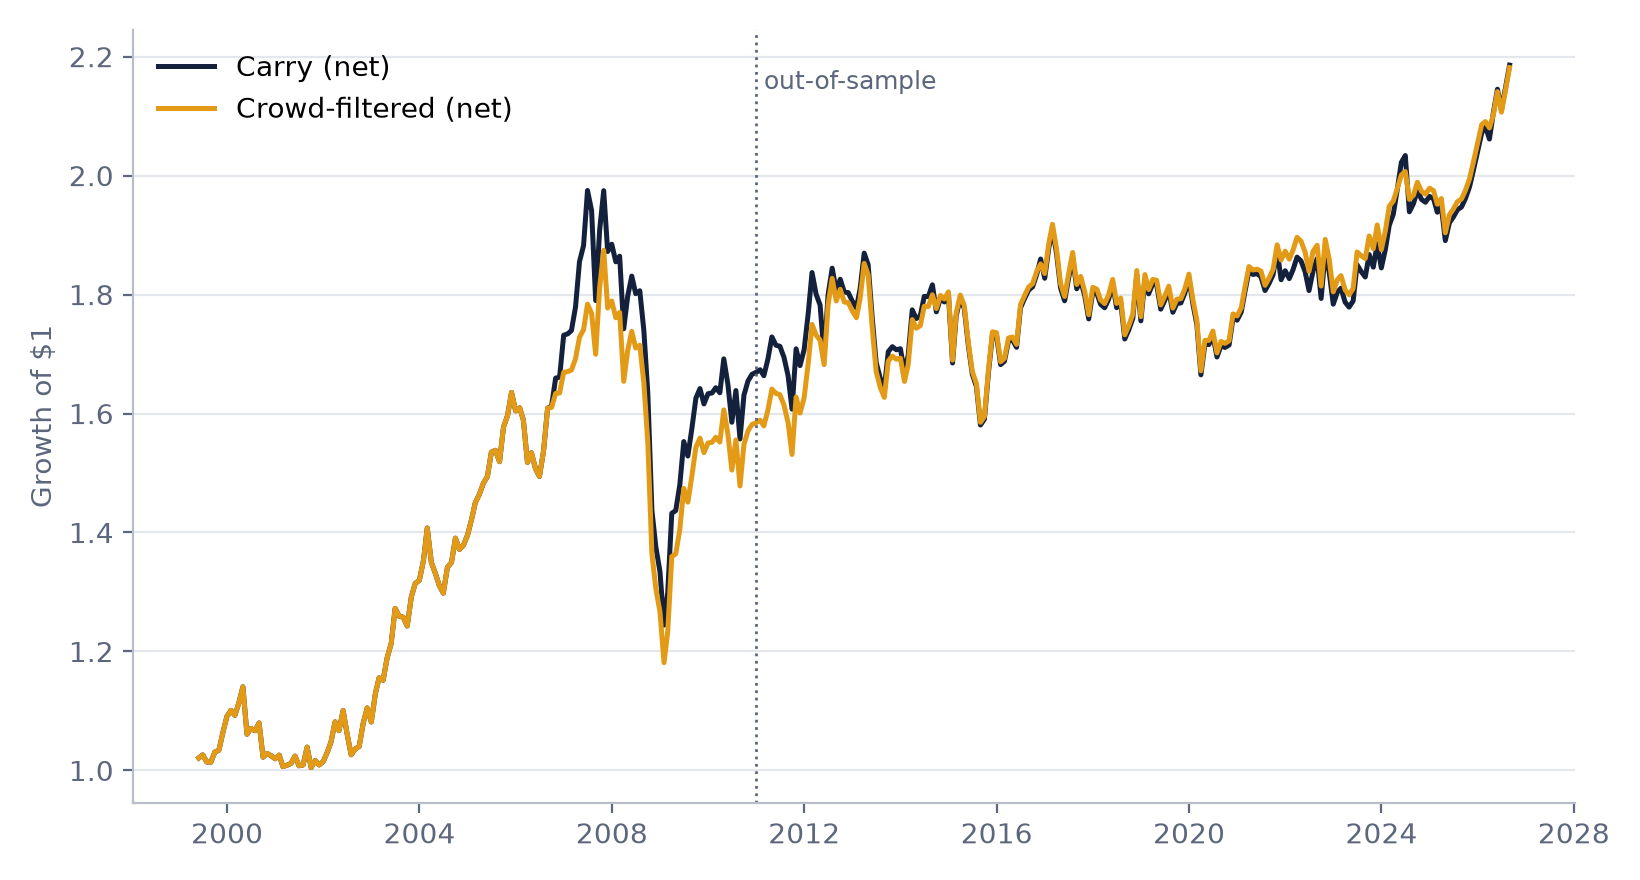
\includegraphics[width=0.85\linewidth]{figures/a_cum.png}
\caption{Strategy A: growth of \$1, carry and crowd-filtered carry (net of costs)}\label{fig:acum}
\tabnote{The figure plots the cumulative value of \$1 invested in plain G10 carry and in crowd-filtered carry, net of 3 basis point costs, from May 1999 to August 2026. The dotted line marks the start of the out-of-sample period in January 2011.}
\end{figure}

Strategy~A closely reproduces the academic carry factor. Over May 1999 to May 2021, its correlation with the \citet{LRV2011} developed-country HML portfolio is 0.82 (Figure~\ref{fig:lrv}). Over this window, Strategy~A earns 3.22\% a year with a Sharpe ratio of 0.34, against 2.34\% and 0.23 for the LRV factor. The evidence supports H-A1.

\begin{figure}[!htbp]
\centering
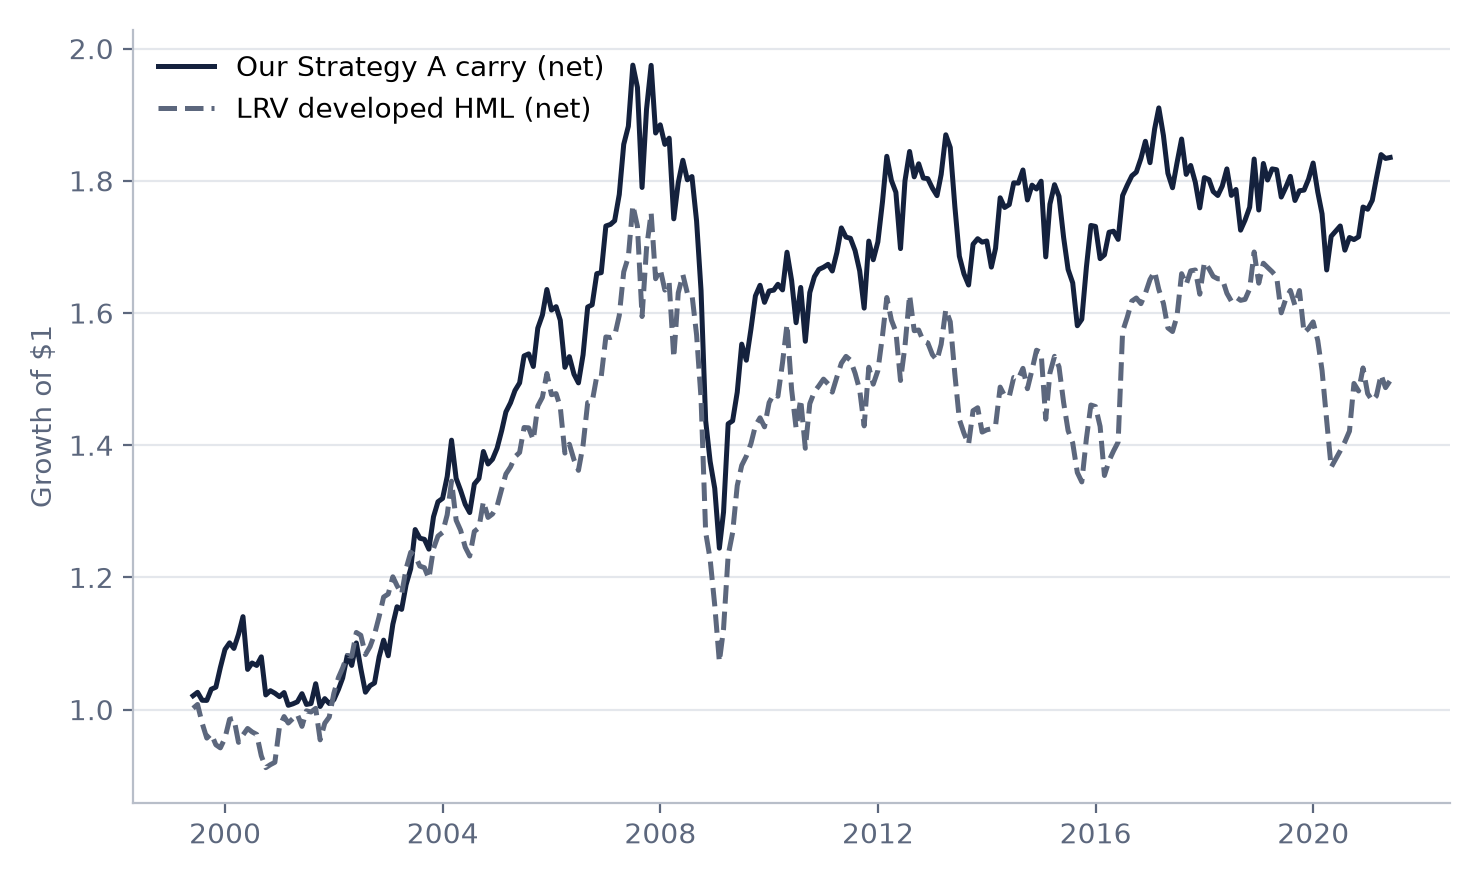
\includegraphics[width=0.8\linewidth]{figures/a_lrv.png}
\caption{Strategy A and the Lustig--Roussanov--Verdelhan carry factor}\label{fig:lrv}
\tabnote{The figure compares the cumulative return of Strategy A (net) with the developed-country high-minus-low carry factor of \citet{LRV2011}, May 1999 to May 2021. The monthly correlation is 0.82.}
\end{figure}

\subsection{Does crowding predict weak carry? (H-A2)}

Table~\ref{tab:crowd} compares carry in the month after crowded and non-crowded readings. After the 295 non-crowded months, carry earns 0.30\% in the next month on average. After the 33 crowded months it earns only 0.02\%, with similar volatility and more negative skewness ($-0.71$ against $-0.46$). The difference is economically meaningful but, with only 33 crowded months, not statistically precise.

\begin{table}[!htbp]
\centering
\caption{Next-Month Carry After Crowded and Non-Crowded Months}\label{tab:crowd}
\small
\begin{tabular}{lcccc}
\toprule
 & Months & Mean (\%) & Volatility (\%) & Skewness \\
\midrule
Not crowded & 295 & 0.30 & 2.56 & $-0.46$ \\
Crowded & 33 & \textbf{0.02} & 2.67 & $-0.71$ \\
\bottomrule
\end{tabular}
\tabnote{This table reports the monthly mean, volatility, and skewness of plain carry returns in month $t+1$, conditional on whether the crowding measure $\text{crowd}_t$ exceeded one at the end of month $t$. Returns are net of costs, May 1999 to August 2026.}
\end{table}

As a trading rule, the crowding filter helps modestly. It leaves the full-sample Sharpe ratio almost unchanged (0.37 to 0.38) but raises the out-of-sample Sharpe ratio from 0.27 to 0.32 and slightly reduces volatility and negative skewness (Table~\ref{tab:A}). Table~\ref{tab:Arob} shows that this improvement is not an artefact of the chosen parameters: every combination of threshold (0.5, 1.0, 1.5) and exposure cut (to 0\% or 50\%) beats plain carry out of sample, with Sharpe ratios between 0.30 and 0.39.

\begin{table}[!htbp]
\centering
\caption{Robustness of the Crowding Filter}\label{tab:Arob}
\small
\begin{tabular}{cccc}
\toprule
Crowding threshold & Exposure when crowded & Sharpe, full sample & Sharpe, out-of-sample \\
\midrule
0.5 & 0\% & 0.37 & 0.31 \\
0.5 & 50\% & 0.38 & 0.30 \\
1.0 & 0\% & 0.38 & 0.37 \\
\textbf{1.0} & \textbf{50\% (pre-specified)} & \textbf{0.38} & \textbf{0.32} \\
1.5 & 0\% & 0.35 & 0.39 \\
1.5 & 50\% & 0.36 & 0.33 \\
\midrule
\multicolumn{2}{l}{Plain carry (no filter)} & 0.37 & 0.27 \\
\bottomrule
\end{tabular}
\tabnote{This table reports net Sharpe ratios of the crowd-filtered strategy for different crowding thresholds and exposure levels. The pre-specified setting is in bold. The grid is reported for robustness and was not used to choose the headline parameters.}
\end{table}

The filter does not, however, avoid the largest crash. The maximum drawdown is $-37$\% with or without it, because the 2008 unwind began from a non-crowded reading. We therefore classify H-A2 as ``leaning yes'': crowding predicts weaker carry on average, but it is not a reliable crash predictor.

\subsection{When does FX carry lose money? (H-A3)}

Table~\ref{tab:Areg} regresses monthly net carry returns on the dollar factor and on equity-volatility innovations. Carry loads positively on the dollar factor (0.35, $t=4.1$) and negatively on volatility shocks ($-1.55$, $t=-3.7$). Together the two factors explain 18\% of the variation in carry returns, and the monthly alpha of 0.25\% is not statistically significant ($t=1.7$). The evidence supports H-A3 and the view of \citet{Menkhoff2012} that carry is compensation for exposure to global volatility risk rather than a free lunch.

\begin{table}[!htbp]
\centering
\caption{Strategy A: Exposure to Dollar and Volatility Risk}\label{tab:Areg}
\small
\begin{tabular}{lcccc}
\toprule
Model & Dollar factor (RX) & Volatility innovation & Monthly alpha (\%) & $R^2$ \\
\midrule
RX only & 0.42 & & 0.26 & 0.12 \\
 & (4.4) & & (1.6) & \\
Volatility only & & $-1.93$ & 0.26 & 0.10 \\
 & & ($-4.3$) & (1.6) & \\
Both & 0.35 & $-1.55$ & 0.25 & 0.18 \\
 & (4.1) & ($-3.7$) & (1.7) & \\
\bottomrule
\end{tabular}
\tabnote{This table reports OLS regressions of monthly net returns of Strategy A on the dollar factor RX and the equity-volatility innovation of \citet{LRV2011}. Newey--West $t$-statistics with three lags are in parentheses. The sample is May 1999 to May 2021 (264 months), limited by the availability of the factor data.}
\end{table}

Figure~\ref{fig:a2008} shows the 2008 episode. From July 2008 to March 2009 the strategy lost 20.5\% as the funding currencies, the yen and the Swiss franc, rallied against the Australian and New Zealand dollars. The worst single months were October 2008 ($-12.0$\%), August 2007 ($-7.8$\%), May 2000 ($-7.0$\%), January 2009 ($-6.8$\%), March 2008 ($-6.5$\%), and January 2015 ($-6.4$\%, the removal of the Swiss franc floor). All are periods of rising global risk aversion or sudden moves in a funding currency.

\begin{figure}[!htbp]
\centering
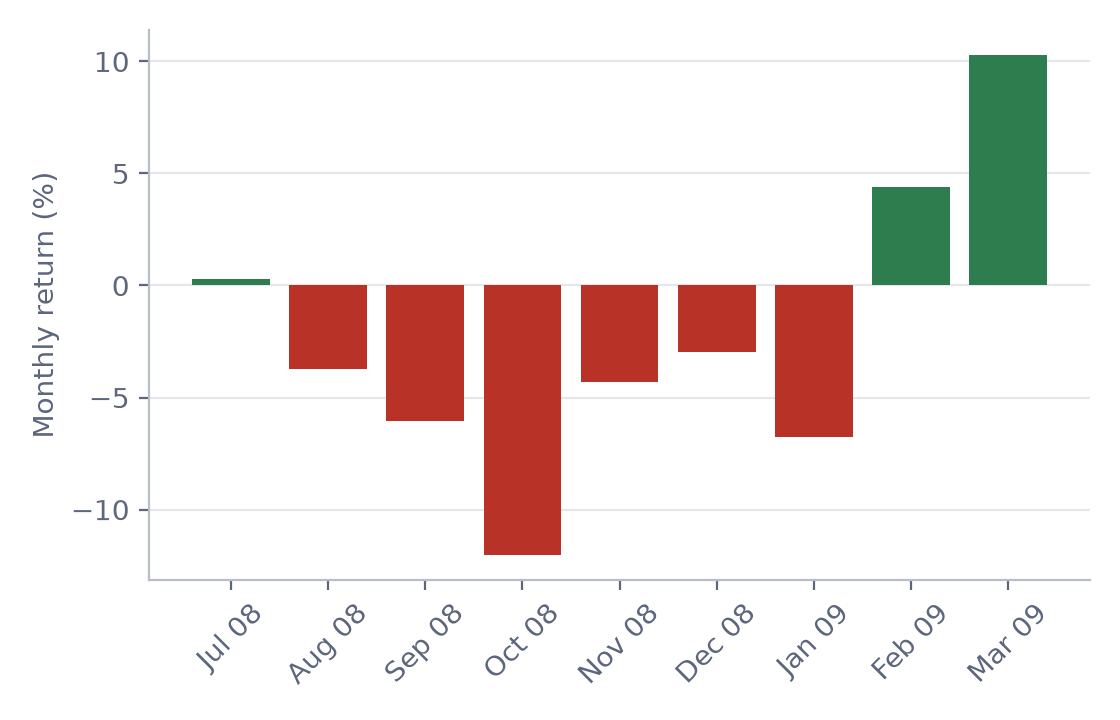
\includegraphics[width=0.62\linewidth]{figures/a_2008.png}
\caption{The 2008 carry crash}\label{fig:a2008}
\tabnote{The figure shows monthly net returns of Strategy A from July 2008 to March 2009, during which the strategy lost 20.5\%.}
\end{figure}

%==========================================================
\section{Results: Crypto Funding Carry}\label{sec:crypto}
%==========================================================

\subsection{Performance and the source of returns (H-C1)}

Table~\ref{tab:C} reports the performance of Strategy~C. Before costs it earns 6.38\% a year with 29.9\% volatility (Sharpe 0.21). Turnover is high, about 45 times capital a year, so costs of 5 basis points take 2.25 percentage points a year, leaving 4.13\% net and a Sharpe ratio of 0.14. The maximum drawdown is $-67$\%. Performance differs sharply between subperiods: the strategy loses money in 2020--2023 (Sharpe $-0.07$) and earns 13.9\% a year with a Sharpe ratio of 0.81 in 2024--2026. Figure~\ref{fig:ccum} plots the growth of one dollar with the main events.

\begin{table}[!htbp]
\centering
\caption{Strategy C: Crypto Funding Carry}\label{tab:C}
\small\setlength{\tabcolsep}{4pt}
\begin{tabular}{llcccccc}
\toprule
 & Period & Mean (\%) & Vol (\%) & Sharpe & Max DD (\%) & Worst week (\%) & Turnover \\
\midrule
Gross & Full 2020:02--2026:08 & 6.38 & 29.87 & 0.21 & $-66.0$ & $-27.2$ & 45 \\
Net & Full & 4.13 & 29.87 & \textbf{0.14} & $-67.3$ & $-27.3$ & 45 \\
Net & In-sample 2020--2023 & $-2.52$ & 36.05 & $-0.07$ & $-67.3$ & $-27.3$ & 45 \\
Net & Out-of-sample 2024--2026 & 13.87 & 17.21 & \textbf{0.81} & $-13.3$ & $-9.2$ & 44 \\
\bottomrule
\end{tabular}
\tabnote{This table reports annualised performance of Strategy C, which every Sunday shorts the third of coins with the highest seven-day average funding rate and buys the third with the lowest, with 50\% of capital in each leg, and holds for seven days. Net returns deduct 5 basis points per unit of turnover. Statistics use daily returns annualised with 365 days. Turnover is annual, in multiples of capital.}
\end{table}

\begin{figure}[!htbp]
\centering
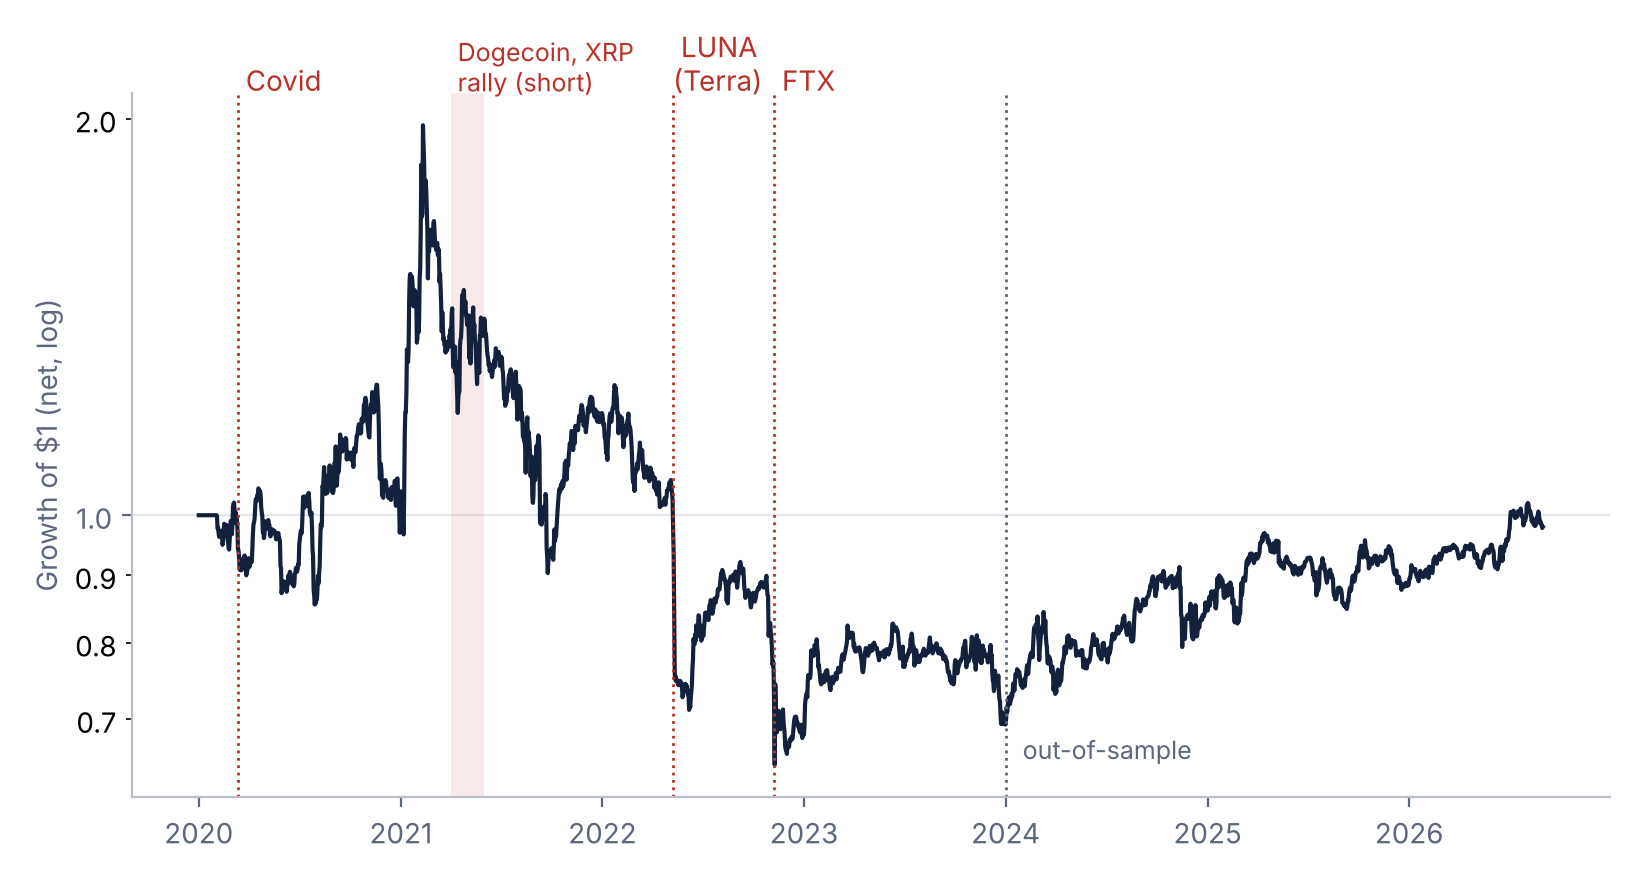
\includegraphics[width=0.85\linewidth]{figures/c_cum_annotated.png}
\caption{Strategy C: growth of \$1 (net of costs, log scale)}\label{fig:ccum}
\tabnote{The figure plots the cumulative value of \$1 invested in Strategy C, net of 5 basis point costs, February 2020 to August 2026. The shaded band marks the Dogecoin and XRP rally of April--May 2021, when the strategy was short both coins. The main collapses (Terra in May 2022 and FTX in November 2022) are marked.}
\end{figure}

Table~\ref{tab:Cdec} decomposes the return. Over the full sample, the strategy collects 8.55\% a year in funding, as H-C1 predicts, but loses 2.17\% a year on price moves and 2.25\% on costs. In 2020--2023 the funding income (12.3\%) was entirely offset by price losses ($-12.5$\%), as the coins the strategy shorted for their high funding, such as Dogecoin and XRP, kept rallying. Since 2024 funding has been lower (3.1\%) and most of the gain came from prices (13.0\%). Figure~\ref{fig:cdec} shows the two components over time. We classify H-C1 as ``mixed'': the strategy collects real funding, but price moves decide the result.

\begin{table}[!htbp]
\centering
\caption{Strategy C: Where the Return Comes From}\label{tab:Cdec}
\small
\begin{tabular}{lcccc}
\toprule
Period & Funding (\%) & Price (\%) & Costs (\%) & Net (\%) \\
\midrule
Full 2020--2026 & 8.55 & $-2.17$ & $-2.25$ & 4.13 \\
In-sample 2020--2023 & 12.26 & $-12.51$ & $-2.27$ & $-2.52$ \\
Out-of-sample 2024--2026 & 3.10 & 12.99 & $-2.22$ & 13.87 \\
\bottomrule
\end{tabular}
\tabnote{This table decomposes the annualised net return of Strategy C into funding received or paid, price returns, and transaction costs, in percent per year.}
\end{table}

\begin{figure}[!htbp]
\centering
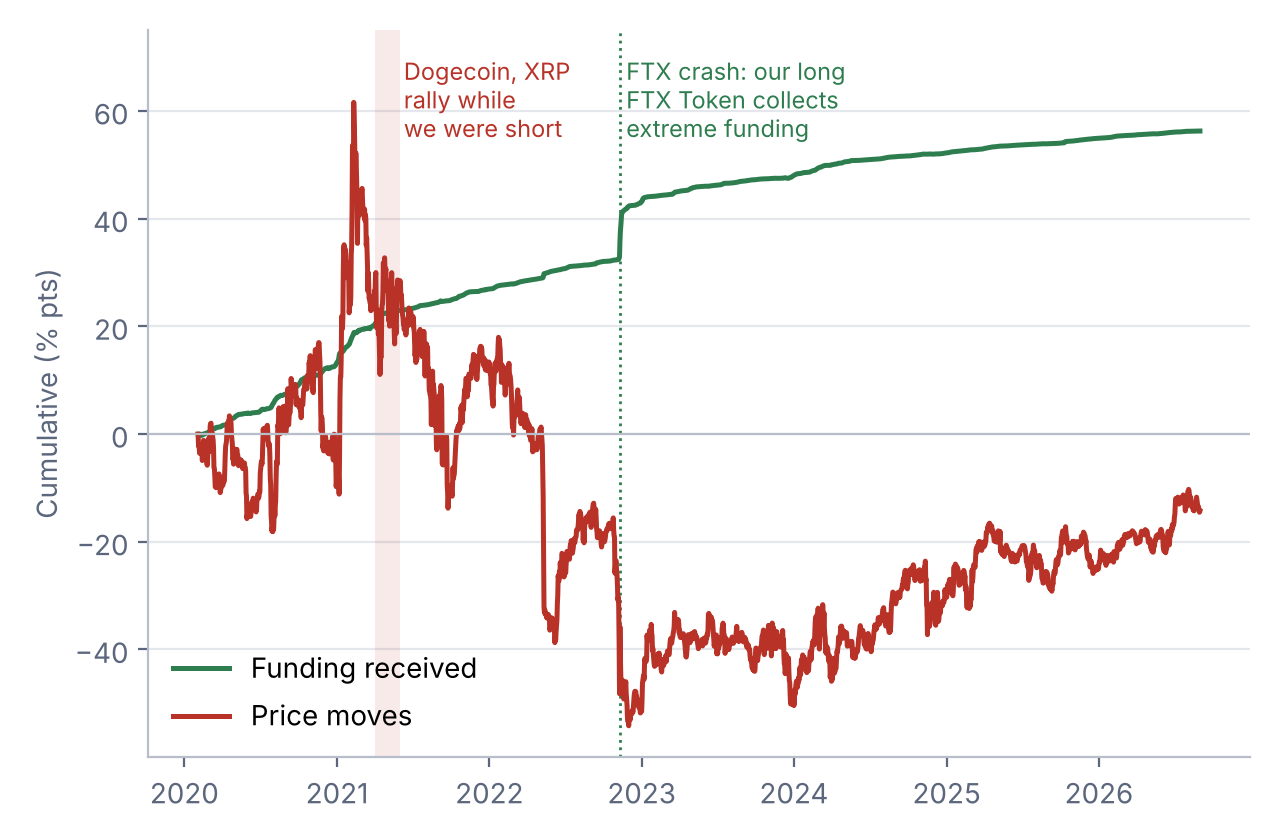
\includegraphics[width=0.72\linewidth]{figures/c_decomp_annotated.png}
\caption{Strategy C: cumulative funding received and price returns}\label{fig:cdec}
\tabnote{The figure plots the cumulative funding and price components of Strategy C. The dotted line marks the FTX collapse in November 2022, when the strategy was long FTX Token and collected extreme funding.}
\end{figure}

Table~\ref{tab:Crob} shows the robustness of Strategy~C to the funding lookback and rebalancing frequency. All six settings have a positive out-of-sample Sharpe ratio (0.41 to 1.29), and the pre-specified seven-day weekly setting lies in the bottom half of the full-sample results. Shorter lookbacks and daily rebalancing perform better even after costs, which suggests that the funding signal decays quickly.

\begin{table}[!htbp]
\centering
\caption{Strategy C: Robustness to Lookback and Rebalancing}\label{tab:Crob}
\small
\begin{tabular}{llcc}
\toprule
Funding lookback & Rebalancing & Sharpe, full sample & Sharpe, out-of-sample \\
\midrule
3 days & Daily & 0.68 & 0.41 \\
3 days & Weekly & 0.49 & 1.29 \\
7 days & Daily & 0.56 & 0.92 \\
\textbf{7 days} & \textbf{Weekly (pre-specified)} & \textbf{0.14} & \textbf{0.81} \\
30 days & Daily & 0.28 & 0.83 \\
30 days & Weekly & 0.07 & 0.42 \\
\bottomrule
\end{tabular}
\tabnote{This table reports net Sharpe ratios of Strategy C for different funding lookback windows and rebalancing frequencies. The pre-specified setting is in bold. The grid was not used to choose the headline parameters.}
\end{table}

\subsection{What drives crypto carry losses? (H-C2)}

Crypto carry has no market exposure. A daily regression on Bitcoin returns gives a beta of $-0.02$ (Newey--West $t=-0.75$) and an $R^2$ of 0.001. Its losses are instead coin-specific. The worst week, ending May 15, 2022, cost 27.3\%. In that week the strategy was \emph{long} Terra: traders were shorting LUNA so heavily that its seven-day funding had turned negative, about $-20$\% a year, and the rule placed it in the long leg just before it collapsed. The other worst weeks ended September 12, 2021 ($-12.3$\%), November 13, 2022 ($-11.6$\%, the FTX collapse), November 29, 2020 ($-11.0$\%), and August 15, 2021 ($-10.0$\%).

Figure~\ref{fig:contrib} shows the total contribution of each coin to the strategy's profit and loss. Four coins account for most of the losses: Terra ($-87$ percentage points), XRP ($-58$), Dogecoin ($-44$), and FTX Token ($-13$). The winners are Solana ($+102$), BNB ($+51$), Avalanche ($+36$), Cardano ($+32$), and Chainlink ($+27$). In every case the price component dominates the funding component.

\begin{figure}[!htbp]
\centering
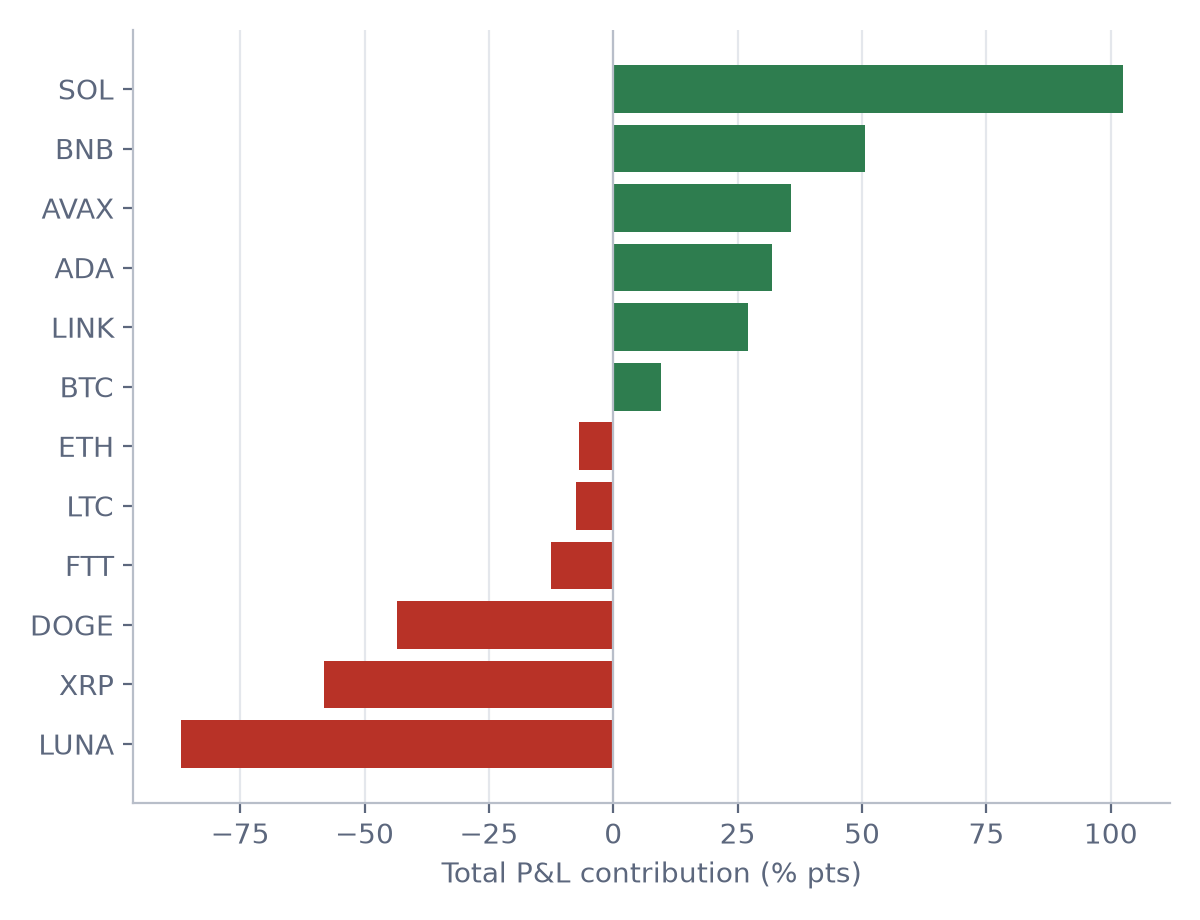
\includegraphics[width=0.62\linewidth]{figures/c_contrib.png}
\caption{Strategy C: total profit and loss by coin}\label{fig:contrib}
\tabnote{The figure shows the cumulative contribution of each coin to the net profit and loss of Strategy C, in percentage points, February 2020 to August 2026.}
\end{figure}

This pattern is the mirror image of FX carry. In FX, carry crashes when a crowded long position in high-yield currencies unwinds. In crypto, the dangerous positions are those in which the strategy takes the other side of a crowd: it is short coins that leveraged traders are crowding to buy (Dogecoin and XRP in 2021), and long coins they are crowding to sell (Terra and FTX Token in 2022). The evidence supports H-C2: crypto carry is market-neutral, but its crashes come from single coins with extreme funding.

%==========================================================
\section{Diversification: Combining FX and Crypto Carry}\label{sec:comb}
%==========================================================

Table~\ref{tab:comb} reports the two strategies scaled to 10\% volatility and their 50/50 combination over February 2021 to August 2026, the period in which both scaled series are available. The correlation between the scaled strategies is 0.11 (0.12 for unscaled monthly net returns over 78 months). The combined portfolio has volatility of 7.0\%, below the 9.3--9.4\% of either part, and a maximum drawdown of $-10.6$\%, smaller than that of either strategy. Because crypto carry was weak over this period, the combination does not beat FX carry alone on Sharpe ratio (0.51 against 0.71). Figure~\ref{fig:comb} plots the three series. The evidence supports H-D.

\begin{table}[!htbp]
\centering
\caption{Combined Portfolio, 2021:02--2026:08}\label{tab:comb}
\small
\begin{tabular}{lccccc}
\toprule
 & Mean (\%) & Vol (\%) & Sharpe & Max DD (\%) & Worst month (\%) \\
\midrule
A (10\% vol) & 6.70 & 9.43 & 0.71 & $-11.0$ & $-7.4$ \\
C (10\% vol) & 0.44 & 9.28 & 0.05 & $-21.4$ & $-10.2$ \\
Combined 50/50 & 3.57 & 6.96 & 0.51 & $-10.6$ & $-5.9$ \\
\bottomrule
\end{tabular}
\tabnote{Each strategy is scaled to 10\% annual volatility using trailing volatility known at $t-1$ (36 months for A, 12 months for C) and the two are combined with equal weights. Statistics are annualised from 67 monthly net returns.}
\end{table}

\begin{figure}[!htbp]
\centering
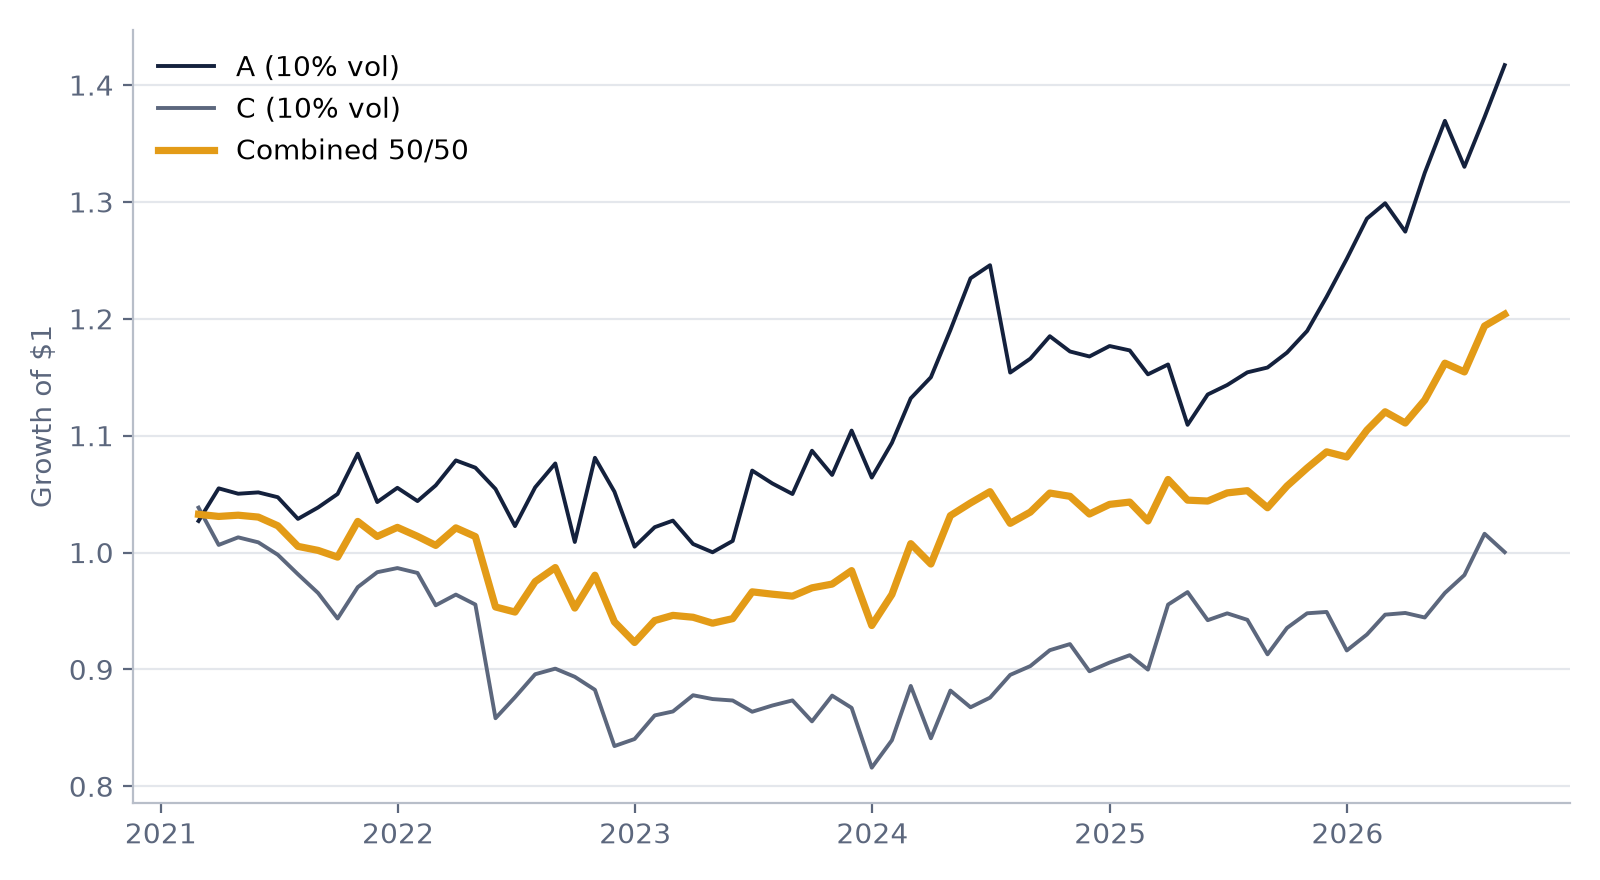
\includegraphics[width=0.85\linewidth]{figures/comb.png}
\caption{FX carry, crypto carry, and the 50/50 combination}\label{fig:comb}
\tabnote{The figure plots the cumulative value of \$1 invested in Strategy A and Strategy C, each scaled to 10\% volatility, and in their 50/50 combination, February 2021 to August 2026.}
\end{figure}

%==========================================================
\section{Discussion}\label{sec:disc}
%==========================================================

Table~\ref{tab:verdict} summarises the evidence on each hypothesis.

\begin{table}[!htbp]
\centering
\caption{Summary of Hypotheses and Evidence}\label{tab:verdict}
\small
\begin{tabular}{p{5.2cm}p{2.2cm}p{7.2cm}}
\toprule
Hypothesis & Verdict & Evidence \\
\midrule
H-A1: G10 carry earns a premium & Supported & Net Sharpe 0.37; correlation 0.82 with the LRV factor \\
H-A2: crowding predicts weaker carry & Leaning yes & 0.02\% vs 0.30\% next month; out-of-sample Sharpe 0.27 to 0.32; missed 2008 \\
H-A3: carry loses in volatility spikes & Supported & Volatility beta $-1.55$ ($t=-3.7$); alpha not significant \\
H-C1: funding carry earns a premium & Mixed & Funding $+8.5$\% a year, but net Sharpe 0.14; price moves dominate \\
H-C2: no BTC exposure; coin-specific crashes & Supported & BTC beta $\approx 0$; Terra $-87$ points; worst week $-27$\% \\
H-D: FX and crypto carry diversify & Supported & Correlation 0.11; combined volatility 7.0\% vs about 9\% \\
\bottomrule
\end{tabular}
\end{table}

\paragraph{Interpretation.}
In foreign exchange, our results agree with the risk-based view of carry. G10 carry earns a modest premium, tracks the academic carry factor, and loses when volatility rises. Crowding measured from CFTC positions adds information: carry is weaker after crowded months, and a simple filter improves out-of-sample performance under every parameter choice we tried. But crowding is a slow-moving signal, and the largest crash in our sample started from a position that did not look crowded. The 2008 unwind was driven by a global funding shock that hit carry whether or not speculators were heavily positioned, consistent with \citet{BrunnermeierPedersen2009}.

In crypto, the funding rate is a direct and fast measure of crowded leveraged demand. Sorting on it collects real income, but it also places the strategy against the crowd on both sides. Being short crowded longs lost money in the 2021 retail rally, and being long crowded shorts lost money in the 2022 collapses. Crowding therefore tells an investor \emph{where} the risk sits rather than \emph{when} it will materialise.

\paragraph{Implications.}
For FX investors, positioning data provide a cheap overlay that modestly improves carry but does not replace hedging against volatility shocks. For crypto, sorting on funding alone exposes a portfolio to single-coin collapses. A better design would react faster (the robustness grid points towards shorter lookbacks and daily rebalancing), treat extremely negative funding as a warning of crowded shorts rather than an opportunity, and size positions by coin-level risk.

\paragraph{Limitations.}
Our results have several limitations. The crypto sample covers about six and a half years and twelve coins, each leg usually holds three coins, and single-coin events dominate. Strategy~C reverses between the in-sample period (Sharpe $-0.07$) and the out-of-sample period (0.81), and the out-of-sample gains came mostly from price moves, so they are not evidence of a stable premium. In FX, only 33 months were crowded, which limits statistical power. Data availability limits the FX sample to start in 1999 and the factor regressions to end in 2021. Finally, transaction costs are proportional estimates; we do not model funding caps, borrowing limits, slippage under stress, or exchange counterparty risk, which was material in the FTX collapse.

%==========================================================
\section{Conclusion}\label{sec:concl}
%==========================================================

We ask whether carry trades crash when they are crowded, using G10 currencies and crypto perpetual futures. Our answer is partly yes. Crowding makes carry weaker, but it does not predict the biggest crashes. In FX, carry crashes are compensation for exposure to volatility risk, and crowding measured from CFTC positions is a modest warning sign rather than a reliable crash predictor. In crypto, carry also earns a premium and also crashes, but the crashes come from single coins, mostly from being long a coin that traders are crowding to short, so crowding tells investors where the danger is rather than when it will hit. Because the two carry trades are nearly uncorrelated, combining them reduces volatility and drawdowns.

Our results suggest two directions for future work: testing faster crowding measures in FX, such as options skew or flow data, and testing in a larger crypto universe whether extreme negative funding predicts collapses.

\clearpage
\setstretch{1.0}
\begin{thebibliography}{99}

\bibitem[Brunnermeier et~al.(2008)]{BrunnermeierNagelPedersen2008}
Brunnermeier, M.~K., S.~Nagel, and L.~H. Pedersen, 2008, Carry trades and currency crashes, \textit{NBER Macroeconomics Annual} 23, 313--347.

\bibitem[Brunnermeier and Pedersen(2009)]{BrunnermeierPedersen2009}
Brunnermeier, M.~K., and L.~H. Pedersen, 2009, Market liquidity and funding liquidity, \textit{Review of Financial Studies} 22, 2201--2238.

\bibitem[Burnside et~al.(2011)]{Burnside2011}
Burnside, C., M.~Eichenbaum, I.~Kleshchelski, and S.~Rebelo, 2011, Do peso problems explain the returns to the carry trade?, \textit{Review of Financial Studies} 24, 853--891.

\bibitem[Daniel et~al.(2017)]{DanielHodrickLu2017}
Daniel, K., R.~J. Hodrick, and Z.~Lu, 2017, The carry trade: Risks and drawdowns, \textit{Critical Finance Review} 6, 211--262.

\bibitem[Fama(1984)]{Fama1984}
Fama, E.~F., 1984, Forward and spot exchange rates, \textit{Journal of Monetary Economics} 14, 319--338.

\bibitem[Farhi and Gabaix(2016)]{Farhi2016}
Farhi, E., and X.~Gabaix, 2016, Rare disasters and exchange rates, \textit{Quarterly Journal of Economics} 131, 1--52.

\bibitem[Hansen and Hodrick(1980)]{HansenHodrick1980}
Hansen, L.~P., and R.~J. Hodrick, 1980, Forward exchange rates as optimal predictors of future spot rates: An econometric analysis, \textit{Journal of Political Economy} 88, 829--853.

\bibitem[He et~al.(2022)]{He2022}
He, S., A.~Manela, O.~Ross, and V.~von Wachter, 2022, Fundamentals of perpetual futures, Working paper, arXiv:2212.06888.

\bibitem[Jurek(2014)]{Jurek2014}
Jurek, J.~W., 2014, Crash-neutral currency carry trades, \textit{Journal of Financial Economics} 113, 325--347.

\bibitem[Koijen et~al.(2018)]{Koijen2018}
Koijen, R.~S.~J., T.~J. Moskowitz, L.~H. Pedersen, and E.~B. Vrugt, 2018, Carry, \textit{Journal of Financial Economics} 127, 197--225.

\bibitem[Liu and Tsyvinski(2021)]{LiuTsyvinski2021}
Liu, Y., and A.~Tsyvinski, 2021, Risks and returns of cryptocurrency, \textit{Review of Financial Studies} 34, 2689--2727.

\bibitem[Liu et~al.(2022)]{LiuTsyvinskiWu2022}
Liu, Y., A.~Tsyvinski, and X.~Wu, 2022, Common risk factors in cryptocurrency, \textit{Journal of Finance} 77, 1133--1177.

\bibitem[Lustig et~al.(2011)]{LRV2011}
Lustig, H., N.~Roussanov, and A.~Verdelhan, 2011, Common risk factors in currency markets, \textit{Review of Financial Studies} 24, 3731--3777.

\bibitem[Lustig et~al.(2014)]{LRV2014}
Lustig, H., N.~Roussanov, and A.~Verdelhan, 2014, Countercyclical currency risk premia, \textit{Journal of Financial Economics} 111, 527--553.

\bibitem[Lustig and Verdelhan(2007)]{LustigVerdelhan2007}
Lustig, H., and A.~Verdelhan, 2007, The cross section of foreign currency risk premia and consumption growth risk, \textit{American Economic Review} 97, 89--117.

\bibitem[Menkhoff et~al.(2012)]{Menkhoff2012}
Menkhoff, L., L.~Sarno, M.~Schmeling, and A.~Schrimpf, 2012, Carry trades and global foreign exchange volatility, \textit{Journal of Finance} 67, 681--718.

\bibitem[Moskowitz et~al.(2012)]{Moskowitz2012}
Moskowitz, T.~J., Y.~H. Ooi, and L.~H. Pedersen, 2012, Time series momentum, \textit{Journal of Financial Economics} 104, 228--250.

\bibitem[Newey and West(1987)]{NeweyWest1987}
Newey, W.~K., and K.~D. West, 1987, A simple, positive semi-definite, heteroskedasticity and autocorrelation consistent covariance matrix, \textit{Econometrica} 55, 703--708.

\bibitem[Pedersen(2009)]{Pedersen2009}
Pedersen, L.~H., 2009, When everyone runs for the exit, \textit{International Journal of Central Banking} 5, 177--199.

\bibitem[Schmeling et~al.(2023)]{Schmeling2023}
Schmeling, M., A.~Schrimpf, and K.~Todorov, 2023, Crypto carry, BIS Working Paper No.~1087, Bank for International Settlements.

\bibitem[Stein(2009)]{Stein2009}
Stein, J.~C., 2009, Presidential address: Sophisticated investors and market efficiency, \textit{Journal of Finance} 64, 1517--1548.

\end{thebibliography}

\clearpage
\setstretch{1.25}
\appendix
\section{Replication}\label{app:rep}

All code and data needed to reproduce the results are in the replication package and at \url{https://github.com/rezazamani2329/currency-crypto-carry}. The scripts in \texttt{code/} run in order: \texttt{01} and \texttt{03} download and clean the FX, CFTC, and Binance data; \texttt{02} and \texttt{04} run the backtests for Strategies A and C; and \texttt{05} runs the factor regressions, coin-level analysis, and the combined portfolio. Running \texttt{SKIP\_DOWNLOAD=1 python run\_all.py} reproduces every table and figure from the cleaned data in \texttt{data/clean/}. Table~\ref{tab:files} maps each table and figure to its source file.

\begin{table}[!htbp]
\centering
\caption{Source Files for Tables and Figures}\label{tab:files}
\small
\begin{tabular}{ll}
\toprule
Table or figure & Source file \\
\midrule
Table II, Figure 1 & \texttt{output/strategyA/performance\_table.csv}, \texttt{monthly\_returns.csv} \\
Table III & \texttt{output/strategyA/crowded\_vs\_not.csv} \\
Table IV & \texttt{output/strategyA/robustness\_grid.csv} \\
Table V & \texttt{output/risk/A\_factor\_regressions.csv} \\
Figure 2 & \texttt{output/risk/A\_vs\_LRV\_HML.csv} \\
Figure 3 & \texttt{output/risk/A\_worst\_months.csv} \\
Table VI, Figure 4 & \texttt{output/strategyC/performance\_table.csv}, \texttt{daily\_returns.csv} \\
Table VII, Figure 5 & \texttt{output/strategyC/return\_decomposition.csv} \\
Table VIII & \texttt{output/strategyC/robustness\_grid.csv} \\
Figure 6 & \texttt{output/risk/C\_contribution\_by\_coin.csv} \\
Table IX, Figure 7 & \texttt{output/risk/combined\_portfolio.csv} \\
\bottomrule
\end{tabular}
\end{table}

\end{document}
